% !Mode:: "TeX:UTF-8"

\chapter{背景}[Background]

虽然目前很多公司都开发了自己的自动驾驶系统,但其使用的技术几乎都是基于计算机视觉,目标检测,目标识别等深度学习、机器学习技术。因此,针对自动驾驶系统的测试技术也是源于深度学习系统的测试技术。其中,在基于深度神经网络的自动驾驶系统中,其神经网络模型将被汽车的各种传感器(雷达、摄像头等)接收到的数据作为输入,经过神经元的运算处理后输出各种驾驶行为(方向盘拐角、刹车信号,速度控制信号等)。下图\ref{as_example}展示了一个机遇卷积神经网络的自动驾驶系统例子,这个系统由输入(摄像头拍摄的图像)、输出层(方向盘拐角)和中间的隐藏层组成。本章主要讲述传统的深度学习测试技术以及目前学术界比较推崇的自动测试技术。

\begin{figure}[h]
    \centering
    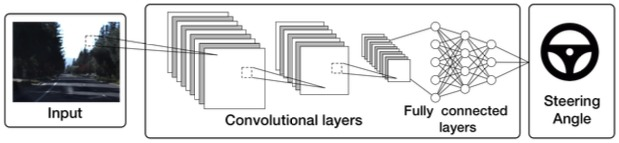
\includegraphics[width=0.8\textwidth]{as_example}
    \caption{基于卷积神经网络的自动驾驶系统\cite{DeepRoad}}
    \label{as_example}
\end{figure}

\section{传统的深度学习系统测试技术}[The traditional testing technology of DNN]

深度学习技术是一种通过研究同类大量数据的表征,对未知新数据的特征进行推测的一门技术。在其行使职能,即预测新数据特征前,必须要学习大量同类的数据,即模型训练。模型训练完成后为了提前检测模型的准确性,会在之前的训练数据集中保留一部分数据,作为训练结束后的模型的测试数据集,使其在未被学习过的测试数据集上进行预测,最后以测试数据集上的准确性作为训练好的模型的精准度。目前学术界公认理想的训练数据集与测试数据集占比分别为70\%和30\%。

% TODO 可扩展

数据集的具体数量跟模型处理的具体问题相关,一般来说,处理的问题越复杂,即数据的特征越多,需要的数据量也就越多,比如比较出名的ImageNet\cite{ImageNet}比赛,公开可用的数据集多达1500万张由人工标注的图片数据。深度学习技术对已有数据特征拟合的本质和其训练测试的过程导致其对数据量的严重依赖,传统的深度学习测试需要大量的人工收集、标注数据,着极度的增加了其中的人力成本。除此之外,传统的通过人工收集数据的方式有严重的缺点,即收集到的数据无法保证覆盖到了所有可能的极端场景,以自动驾驶测试数据集为例,人工收集的数据集一般是车载记录仪记录的道路驾驶视频图片,但一般大雨、大雪等极端天气场景数据很少也很难收集,这就给相应的极端场景自动驾驶系统测试带来了不确定性。

\section{DeepXplore、DeepTest和DeepRoad}[DeepXplore DeepTest and DeepRoad]

针对上诉问题,DeepXplore和DeepTest提出了深度学习系统测试用例自动生成系统来缓解深度学习系统对于数据量的依赖。

\subsection{DeepXplore}[DeepXplore]
DeepXplore首先指出了深度学习系统与传统的软件开发系统的不同:传统软件的开发人员直接指定软件系统的逻辑,然而深度学习则是从数据特征中“学习、推到”它们的运行规则,甚至对于深度学习系统的开发人员来说,他们都不一定清楚训练好的深度学习模型的确切运行逻辑。因此DeepXplore
不是直接寻找深度学习系统中的逻辑错误,而是通过自动产生、寻找一些能使多个同类深度学习系统做出不同行为判断的测试用例,然后并将这些找到的测试用例放回原训练数据集里重新训练模型,试图修正之前错误的行为

除了将使不同的DNN系统做出不同预测行为为目标外,DeepXplore也借鉴了传统软件测试技术中的代码覆盖率的概念,为了使得尽可能测试整个DNN系统,DeepXplore引入了神经元覆盖率的概念,即测试用例测试过程中,在整个深度学习系统中,被“激活”,即输出值超过了某个阀值,的神经元的个数占整个网络结构神经元总数的占比。与代码覆盖率类似,我们期望神经元覆盖率越高越好。

DeepXplore以神经元覆盖率和使得不同DNN系统输出不一致为目标,将在原始测试用例上的修改抽象成为一个优化算法,使用梯度上升算法,最后自动生成一些使得被测的DNN系统得到不同的预测值,且各个DNN系统的神经元覆盖率很高的测试用例,下图\ref{xplore-wf}是DeepXplore的工作原理图。

\begin{figure}[h]
    \centering
    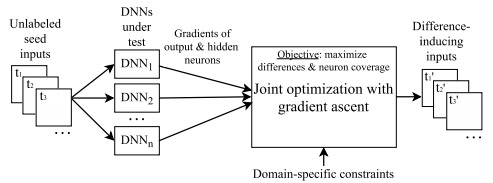
\includegraphics[width=0.8\textwidth]{xplore-wf}
    \caption{DeepXplore工作原理图\cite[图~5]{DeepXplore}}
    \label{xplore-wf}
\end{figure}

\subsection{DeepTest}[DeepTest]

DeepTest基于DeepXplore的工作,提出了一套专门针对自动驾驶系统,能够自动检测出错误行为的测试系统。发生在自动驾驶系统上的车祸大部分都是发生在一些罕见的路况场景下,而传统的自动驾驶检测测试技术几乎是完全依赖大量的罕见路况场景图片的人工收集与标注,这不仅包含了大量的人工成本,重要的是人工收集的数据无法保证能够覆盖度到了所有的极端场景数据。这些极端场景就好像是传统软件中的bug,但是这些bug一旦被检测到,就可能通过把这些导致错误的输入重新放入训练集,同时改变一下模型的结构和参数来修复。DeepTest正是通过以上的思路来设计的一套自动测试系统。

\begin{algorithm}[h]
    \small
    \SetAlgoLined
    \SetKwInOut{Input}{Input}
    \SetKwInOut{Output}{Output}
    \SetKwInOut{Variable}{Variable}

    \Input{变换Transformations T, 种子图像Seed Images I}
    \Output{合成的测试数据图像}
    \Variable{S: 存储新合成图像的栈; Tqueue: 存储变换的队列}

    push all seed imgs to Stack S; 所有种子图片入栈\;
    $genTests = \varnothing$\;
    \While{S is not empty}{
        img = S.pop()\;
        $Tqueue = \varnothing$\;
        numFailedTries = 0 \;
        \While{$numFailedTries \leq maxFailedTries$}{
            \eIf{$Tqueue\ is\ not\ empty$}{
                T1 = Tqueue.deque()
            }{
                Randomly pick transformations T1 from T
            }
            Randomly pick parameter P1 for T1\;
            Randomly pick transformation T2 from T\;
            Randomly pick parameter P2 from T2\;
            newImage = ApplyTransforms(image, T1, P1m T2, P2)\;
            \eIf{covInc(newiamge)}{
                Tqueue.enqueue(T1)
                Tqueue.enqueue(T2)
                UpdateCoverage()
                $genTests=genTests \cup newiamge S.push(newImaghe)$
            }{
                $numFailedTries=numFailed++$
            }
        }
    }
    return genTests
    \caption{混合变换优化算法\cite{DeepTest}}
    \label{alg1}
\end{algorithm}

具体的实现上,DeepTest依旧借用DeepXplore提出的神经元覆盖率的概念,使用位移、拉伸、仿射以及直接修改像素的透明度等基本的图形变换的手段来合成新的驾驶图像,文章里提到合成后的数据能使原DNN系统的神经元覆盖率提升100\%\cite{DeepTest},并以提升神经元覆盖率为目标,给出了一个优化算法\ref{alg1},以获得最佳的图像混合变换,最后DeepTest在利用这些合成的新数据重新训练自动驾驶模型来提高模型对于极端场景的鲁棒性。

\subsection{DeepRoad}[DeepRoad]

尽管DeepTest已经提出了一个较为完善的自动驾驶系统测试方案,以相对便宜和简洁的方法,利用大量的原始和合成出来的驾驶场景图片成功地检测出了许多自动驾驶系统前后不一致的驾驶行为,但它有一个很严重的缺陷:DeepTest用来合成图片的技术很难合成一些能够精确反映现实驾驶场景的图片,并且现实驾驶场景的图片也很难由一些基础的仿射、位移变换模拟合成出来,其用来模拟雨天、雾天的场景的技术仅仅是在原始图层上添加一层额外的图层,如下图\ref{deeptest_effect}所示,对于雾天,DeepTest仅仅是加了一层白色的图层,对于雨天,加了一层线条层。很明显这些合成图离现实中真实的驾驶场景有较大的差别。从另一个角度来说,即时用这些图检测出了自动驾驶系统错误的驾驶行为也很难有说服力,因为这些“出错”的场景在现实中根本不会出现。其实很多可能的真实的驾驶场景根本不能用一些简单的图像处理技术来模拟合成。

\begin{figure}[h]
    \centering
    \subfigure[DeepTest]{
        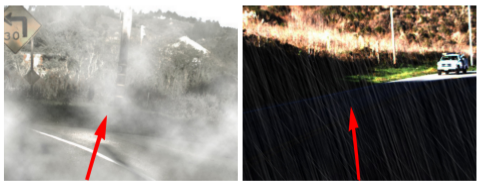
\includegraphics[width = 0.7\textwidth]{deeptest_effect}
    }
    \subfigure[DeepRoad]{
        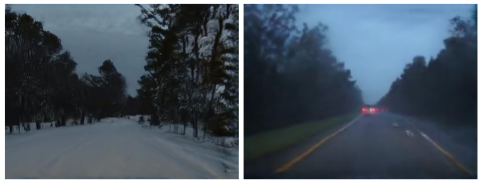
\includegraphics[width = 0.7\textwidth]{deeproad_effect}
    }
    \label{deeptest_effect}
    \caption{天气场景合成效果图比较}
\end{figure}

为了能够自动地合成大量真实的驾驶场景图片,DeepRoad提出了一个半监督合成的框架,抛弃了DeepTest用到的简单的图像处理技术来合成图像,采用深度学习对抗生成网络的技术来合成相对较真实的驾驶场景图片,上图\ref{deeptest_effect}为DeepTest合成图和DeepRoad使用对抗生成网络中UNIT\cite{UNIT}框架合成图的效果对比。可以清楚的看到使用UNIT技术合成的效果比较好的驾驶场景图已经与真实场景很接近了。下图\ref{deeproad_wf}展示了DeepRoad框架的整体流程。 

\begin{figure}[h]
    \centering
    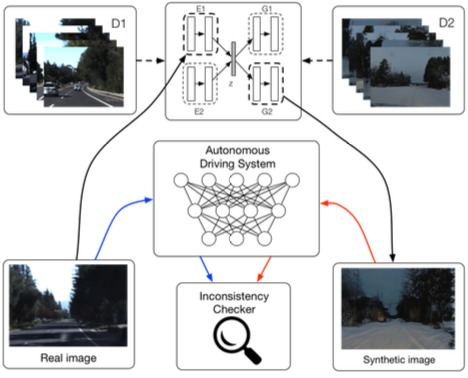
\includegraphics[width=0.75\textwidth]{deeproad_wf}
    \caption{DeepRoad框架流程图\cite{DeepRoad}}
    \label{deeproad_wf}
\end{figure}

DeepRoad将两种天气情况下的图片作为训练输入数据集,训练无监督对抗生成网络UNIT\cite{UNIT}框架,然后利用训练好的UNIT框架对未知新的输入数据进行转换合成,最后测试自动驾驶系统对使用UNIT进行转换后的图片做出的驾驶行为与未转换之前的原始图片的驾驶行为是否一致。

\section{其他的图像转换技术}[Other Image Transformation Technologies]

DeepRoad提出的将深度学习技术运用到自动驾驶系统测试用例合成,并设计的一套自动测试的框架在检测自动驾驶系统的稳定性和鲁棒性上,在其实验检测出了大量的现实自动驾驶系统有误的驾驶行为的结果\cite{DeepRoad}上看是有效的。其相对前人的工作DeepTest主要的改进是将测试用例的合成技术,即驾驶场景的图像转换技术,由原有的基本的图像变换换成了深度学习中的对抗生成网络技术。我们在利用UNIT合成驾驶场景图的实验过程中发现,虽然有效果比较好的合成图,但其占总的合成图的比例很小,1万张结果图中比较真实的图像大约有30多张,大部分的结果图如下,可以看到效果比较差,我们分析了效果比较差的原因主要是使用的训练数据集是由我们从Youtube上爬取的视频制作的数据图像,与UNIT官方使用的NVIDIA公司提供的闭源数据集相差比较大导致。

但其实目前学术界和工业界已经提出的能够进行不同天气场景图像转换的深度学习技术有很多,我们进行了调研,发现主要有两大类:对抗生成网络和图像风格转换(Neural Style Transfer)。我们对DeepRoad进行的实验也表明在得不到理想的训练数据集的情况下利用UNIT进行图像转换的实验结果是不理想的,那么可否将UNIT更换为其他的能够进行图像转换的深度学习技术?哪一种技术的实现效果是最好的?如何评价各种图像转换技术在合成驾驶场景图上的好坏?哪一种技术的训练成本和实现成本是最小的?针对以上问题,我们对现有的能够实现图像风格转换的深度学习技术展开实证研究,希望能够找到答案,最终可以为以后的自动驾驶系统测试人员在选择驾驶场景图片测试用例的合成技术框架上提供一些有帮助的建议。

% TODO UNIT图像

% word count ~ 3450

\chapter{实验}[Methodology]

% metrics -> intro of every gan and experiment, show results

为了尽可能地对所有能够实现图像风格变换的深度学习框架进行试验结果对比,我们首先调研了目前对图片合成图质量的量化评价指标,结合测试人员在实际测试过程中的各种成本以及实验细节,我们总结出了了3个指标: \textit{Fre ́chet Inception Distance(FID)}\cite{FID},模型训练时长以及自动驾驶系统对于前后合成图行为判断方向盘拐角差。

\section{评价指标}[Metrics]

对于图像驾驶场景合成图的质量好坏,最直观也是最直接的方式就是比较合成图的视觉效果,但这种人为的评判是主观且十分容易误判的。为了能够客观、量化的比较各个DNN框架合成的驾驶场景图的好坏,学术界提出了两个指标:\textit{Inception Score(IS)}\cite{IS}和\textit{Fre ́chet Inception Distance(FID)}\cite{FID}。

\textbf{Inception Score(IS).\cite{IS}}\quad IS评价合成图片质量是基于以下两点:(i) 包含有意义的物体图像的条件标记分布应该具有较低的熵(entropy)和(ii) 图像的多样性应该较高,进而边缘分布$\int_z p(y|x=G(z))dz$应该有较高的熵。
将以上两点汇总成一个评分,
\begin{center}
    $IS(G)=\exp{(E_{x\sim G}[d_{KL}(p(y|x), p(y)])}$
\end{center}
IS的作者用ImageNet\cite{ImageNet}的数据训练了一个分类器,最终实验结果反映IS的分数与人工标注评价正相关。

\textbf{Fre ́chet Inception Distance(FID).\cite{FID}}\quad FID提出了另一个评价方法,它首先将所有的合成图片放入一个特征空间,然后将该空间视为一个多元高斯分布,分别计算合成图和真实图的均值与方差,将两者高斯分布的Fre ́chet距离来量化真实图与合成图之间的距离,进而作为对合成图的评价:
\begin{center}
    $FID(x,g)=||\mu_x-\mu_g||_2^2+Tr(\sum_x + \sum_g - 2(\sum_x\sum_g)^{\frac{1}{2}})$
\end{center}
这里的$(\mu_x,\sum_x)$和$(\mu_g,\sum_g)$分别是数据分布和模型分布的均值和方差。FID的作者发现FID值与人类对合成图像的判断一直,并且较IS\cite{IS}鲁棒性更强。相对于IS,FID还能检测出不同类之间的区别,即如果每一种类别值产生合成一张图片,则很有可能获得比较高的IS分数,但对应的FID值却很低。基于以上几点,我们选用FID值而不选择IS值作为我们后面实验评价合成图片质量的评价指标之一。

\textbf{模型训练时长.}\quad 除了直接比较合成图片质量的好坏,在实际的自动驾驶系统测试过程中,我们还必须考虑到模型的训练时长。在选择理想的图片合成框架时,除了最终合成图片质量的好坏,我们还希望模型的训练时间成本尽可能的小,不同的模型根据不同的训练数据集大小,最终的训练时长也相差越大,比如本章后面会提到的UNIT\cite{UNIT}基于Udacity自动驾驶数据集\cite{udacity_dataset}和大约3000张驾驶场景图片,训练50万次时长大约一周左右。而对于一些图像风格转换(Neural Style Transfer)模型来说,训练时长却只要几个小时,虽然最后合成图的质量不如UNIT,但我们希望把这些数据都统计出来,具体的取舍留给实际最终的测试人员自己选择。 

\textbf{方向盘拐角差.}\quad 有了合成图质量的量化指标,模型的训练时间成本比较,最后我们还希望直观地看到合成图相比原始图对于自动驾驶系统行为判断(方向盘拐角信号)的影响。理想情况下,只变换驾驶场景图片的风格,比如晴天的路况转换为夜晚、雨天或者阴天的路况,自动驾驶系统对于大部分的转换后的图像的行为判断,即输出的方向盘拐角信号,与原始的驾驶路况图片做出的行为判断应该几乎一致,或者差别不大。实验中我们对两者的信号,即拐角差设置了一个阈值$\alpha=5^{\circ}$,我们希望小于阈值的图片占比越小越小,最后我们以两者之间拐角差的方差作为该指标的量化数据。

% wc ~ 1400

\section{模型的筛选与实验}[Model Filting and Experiment]


\chapter{发现}[Findings]

\chapter{相关研究}[Related Work]

\chapter{结论}[Conclusions]